\documentclass[../report.tex]{subfiles}
\begin{document}
\graphicspath{{img/}{../img/}}

\section{Overview}
This chapter will describe important implementation details of OCon. The system is realized by three main components. A central, a widget and a client. In addition a communication library have been created to facilitate distributed communication between the three components.


\section{Encapsulation of Context}

Entities are generalized by the interface IEntity, specifying general information for all entities. AbstractEntity extends on IEntity and overrides ToString() with a meaningful implementation. Both are public and it is up the an implementer which to extend.

On figure \ref{fig:PersonImplementation} is extended a Person with property present motivated by the need for this context information.


\begin{figure}[H]
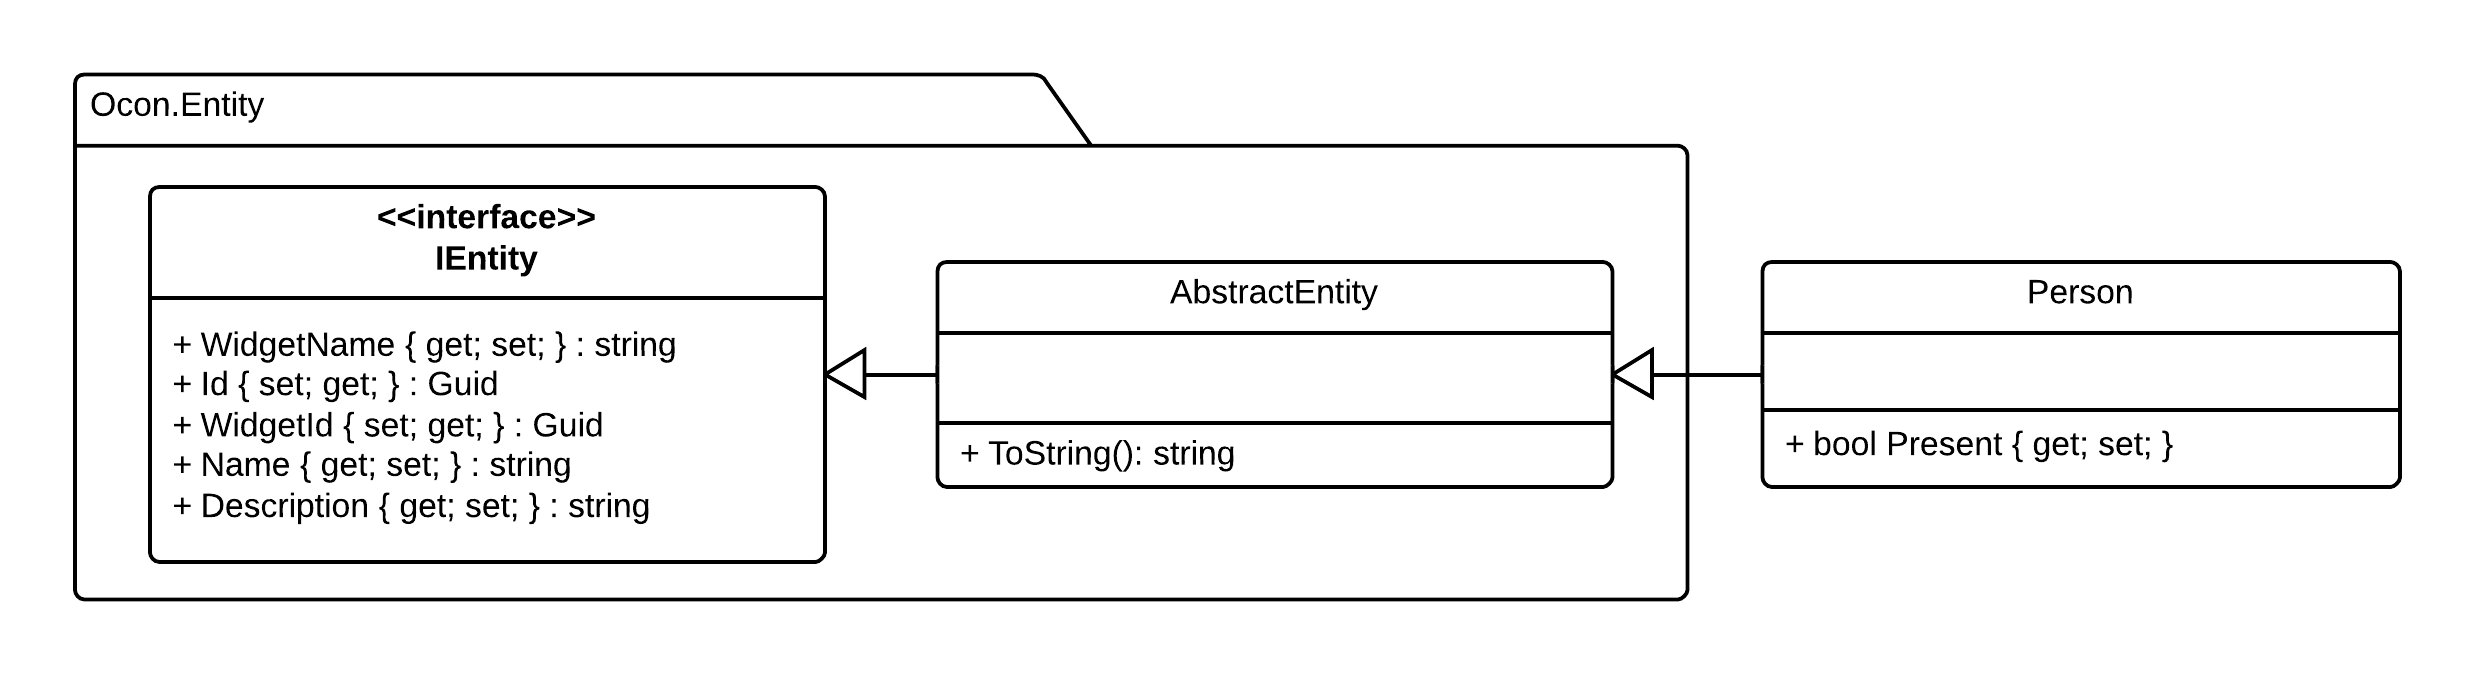
\includegraphics[width=\linewidth]{customEntityClass.png}
\caption{Person as a custom IEntity implementation}
\label{fig:PersonImplementation}
\end{figure}



\section{Situation predicate evaluation}
%\todo{Short on how we evaluate predicates} %

Situations are evaluated on their predicate property. When we say predicate we are talking about the .NET implementation, which is a delegate\footnote{http://msdn.microsoft.com/en-us/library/900fyy8e.aspx} returning a boolean value. The signature for our predicate is as below. This means that a method taking an ICollection of IEntity and returning a boolean can be assigned to the predicate property.

\begin{center}
\texttt{Predicate<ICollection <IEntity> >}
\end{center}


This way it is totally up to an implementor to design the code that evaluates whether a predicate is true or false.


\section{Widget}
\label{sec:OconWidget}

The widget's purpose is to track entities and keep them updated in the central. The widget developer should translate sensor input to entities and then the OCon widget will facilitate tracking the entity and sending it to the central. (See figure \ref{seqwidget})

When the widget is invoked with an entity from the sensor it is checked weather or not the entity is already tracked. If not tracked it will be allocated a new GUID before it is sent to the central. The GUID is a unique ID used for distributed systems and allows OCon to distinguish between adding the entity as a new entity or updating an entity already know to the framework.

\begin{figure}[h]
\centering
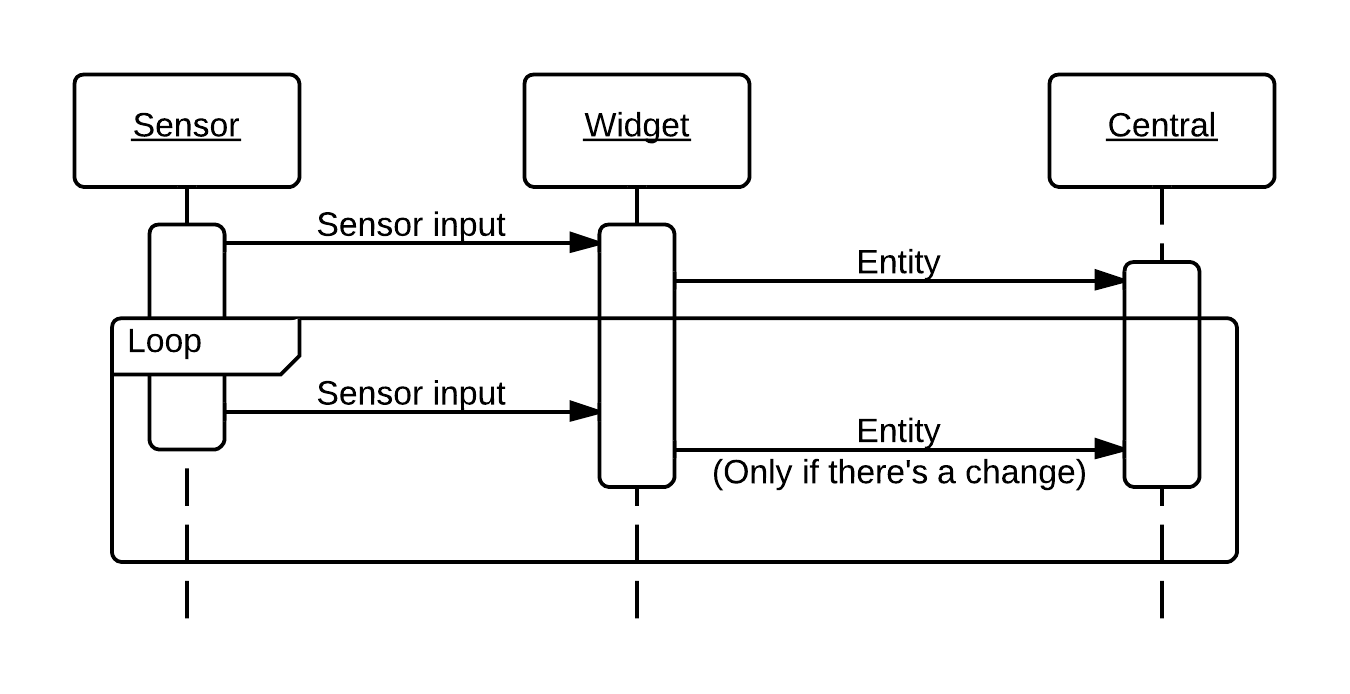
\includegraphics[width=\linewidth]{sequencediagram-widget.png}
\caption{Information flow from Widget to central}
\label{seqwidget}
\end{figure}


\section{Central}
OconCentral is the core component of the framework. Utilization simply means instantiation and afterwards registration of situations.

The OconCentral implementation is a simple binding from the ContextCentral to the ICommunication implementation, making it possible for a developer to use the OconContextFilter in isolation. The OconContextFilter handles all tracking of entities, situations and checking of predicates. Entities are stored in a HashSet<> with a custom EqualityCompare implementation so that the Guid acts as unique identifier. This is necessary for updating informations on entities, but a consequence is that a widget implementation needs to track it's entities as well, to be able to update them with the filter. Evaluation of situation predicates happens whenever an entity is requested tracked.


\section{Client}

The client's purpose it to sent predicates to the central for tracking. When a situation update is send from the central the client must be able to notify the parent application about the situation update. (See figure \ref{seqclient})

\begin{figure}[h]
\centering
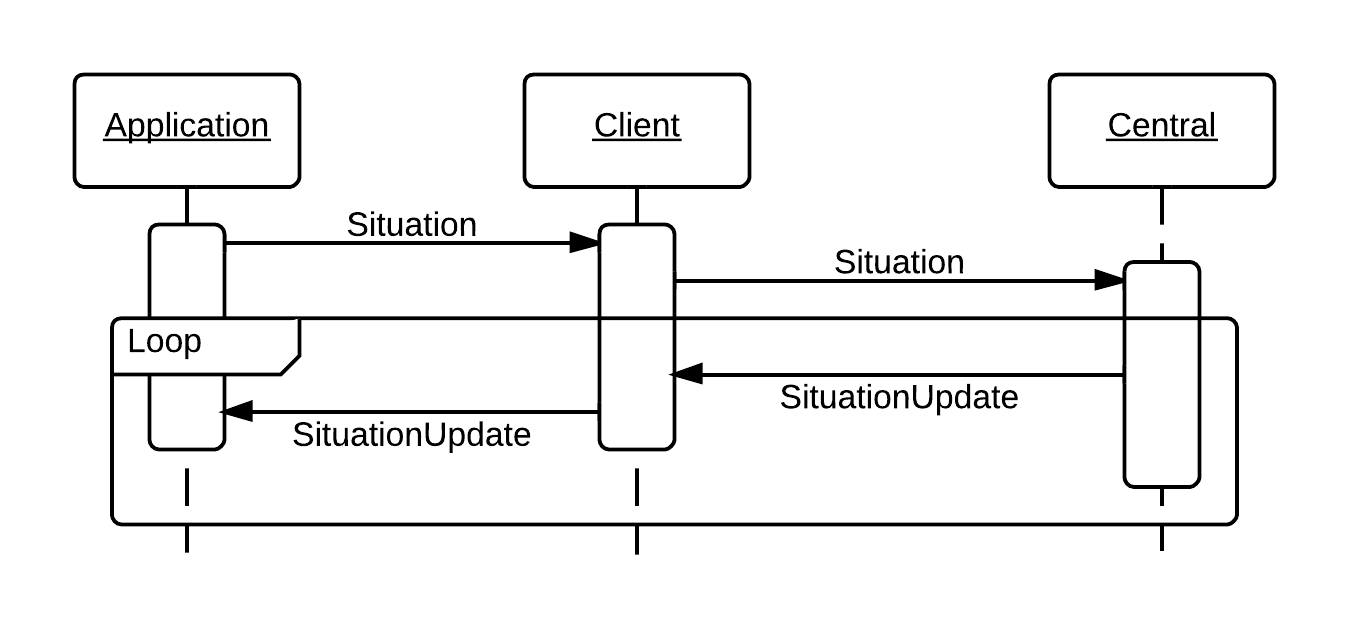
\includegraphics[width=\linewidth]{clientsequencediagram.png}
\caption{Information flow between client and central}
\label{seqclient}
\end{figure}

When the central is discovered the client will send its situations to the central. The central will compute the situation state and sent it back. Whenever the situation state changes the central will sent an update to the client containing the situations new state. The client will then fire an event which the application can listen and react to.

\section{Communication}

To support the design decision that the communication part should be injectable the communication have been interfaced.

OCon contains a default communication implementation build using the TCP/IP layer. For serialization we have chosen to use json. These decisions have been made so that developers are not bound to the .NET platform and can make clients and widgets in other languages like Java, or C directly on a micro controllers like Arduino.

For peer discovery we have chosen to use IP multicast. The central broadcasts itself for peers to discover. The peer, clients and widgets, is listening on the multicast endpoint and will invoke an event when a central is discovered.

The communication subsystem is a vital part of OCon as all communication between peers will go though the subsystem. See figure \ref{fig:widgetComHelper} and \ref{fig:clientComHelper} for a detailed view of the communication between client and central and widget and central.

Just like entities, peers are assigned a GUID. The GUID is an unique identifier for the peer and the communication class stores the IPEndPoints associated with the GUIDs. By doing this messages can be sent only by using the GUID and not the IPEndPoint which adds an abstraction layer to the subsystem.

To support clients being able to sent predicates to the central we must be able to serialize Predicates, but this is unfortunately not supported in .NET. Frameworks for handling the serialization have been researched, but none of the investigated frameworks was able serialize the predicates in OCon as custom types are used. Therefore serializing the predicate was forced out of scope. Instead of sending the predicate, predicates is hard coded in the central. The client can then subscribe them by sending a predicate identifier. This limits the usage of OCon, but it was not possible to include this feature in this project. A framework for serializing the predicates as expression trees should be doable, but that project is left for a later iteration of OCon.

\begin{figure}[h]
\centering
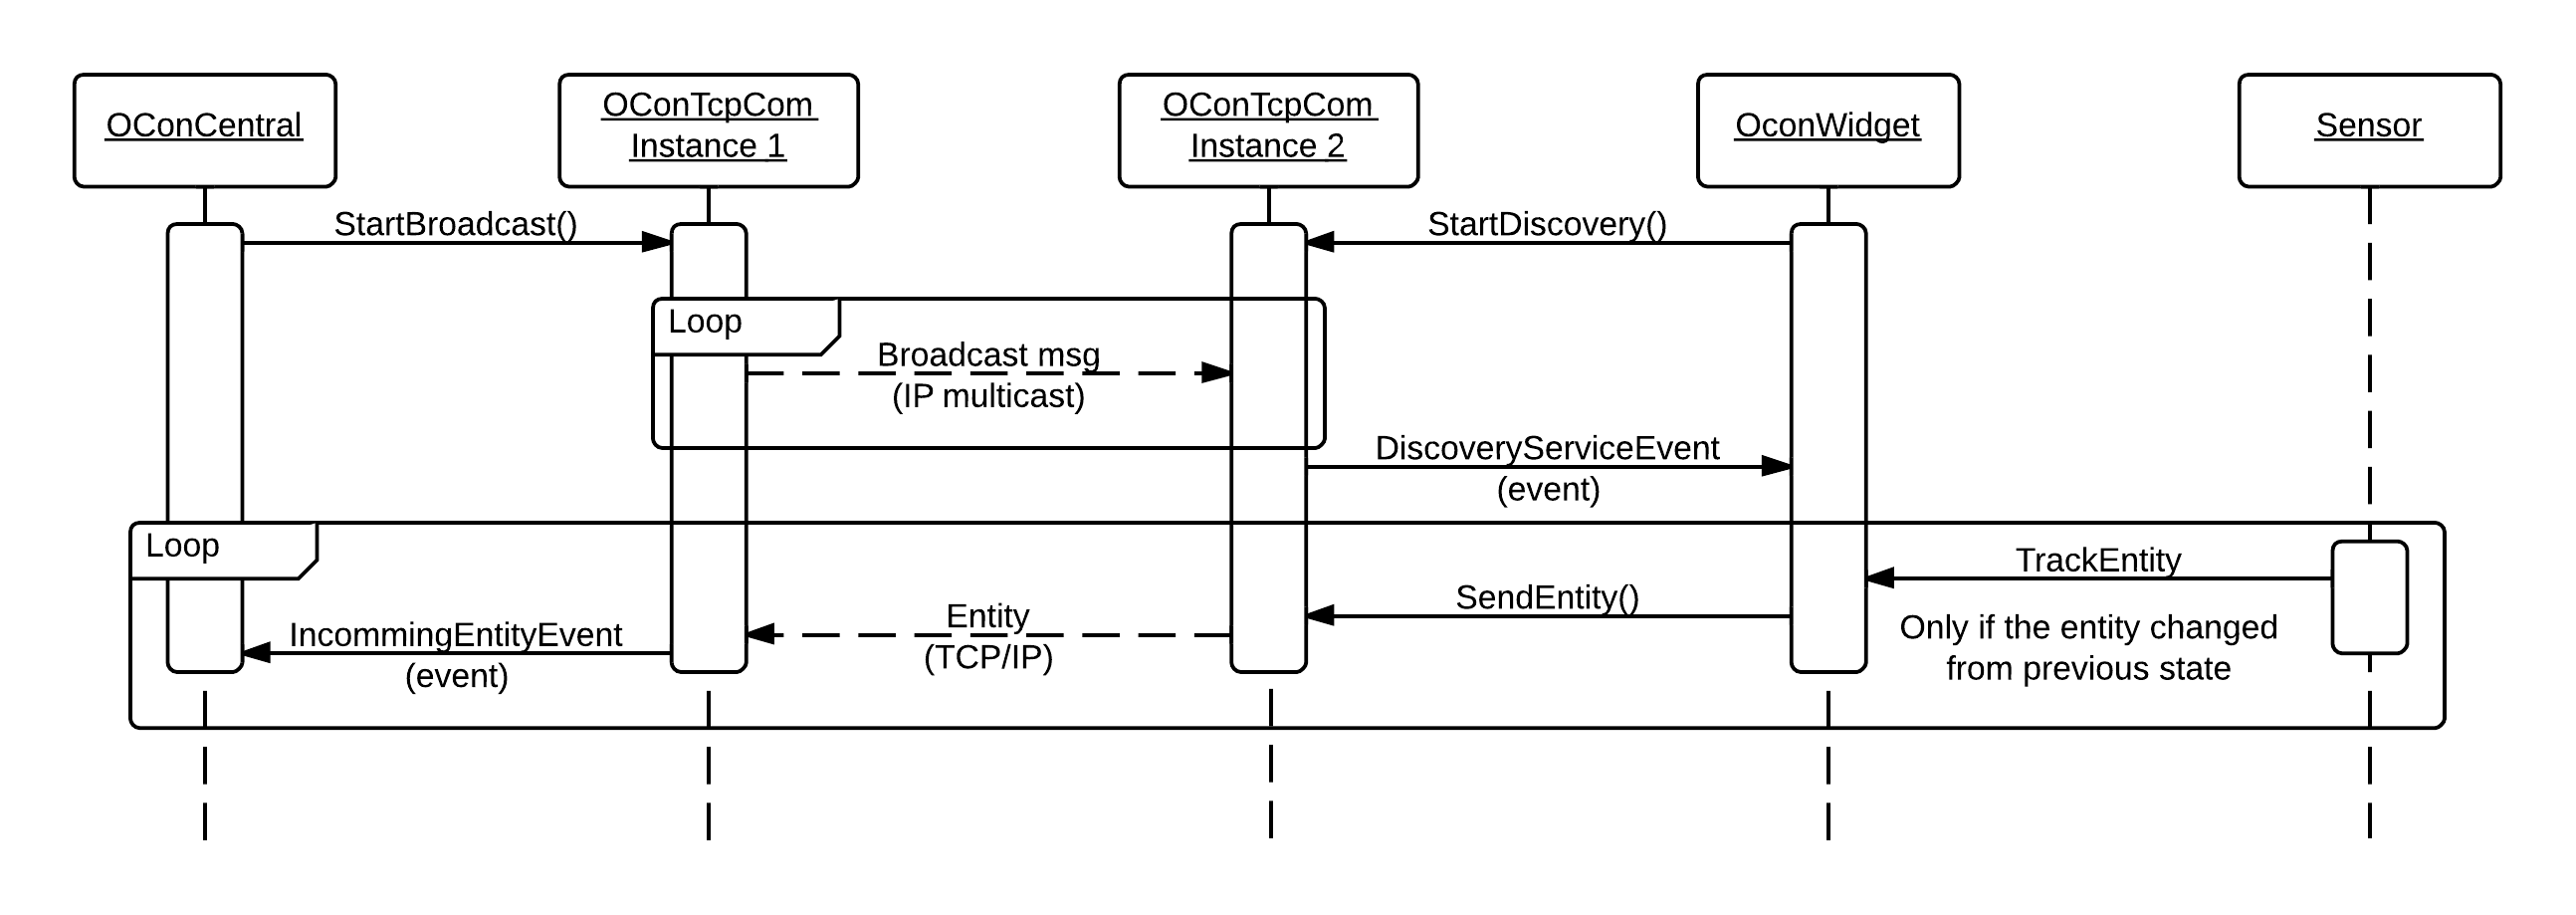
\includegraphics[width=\linewidth]{comHelperSequence-widget.png}
\caption{Widget to Central sequence diagram}
\label{fig:widgetComHelper}
\end{figure}

\begin{figure}[h]
\centering
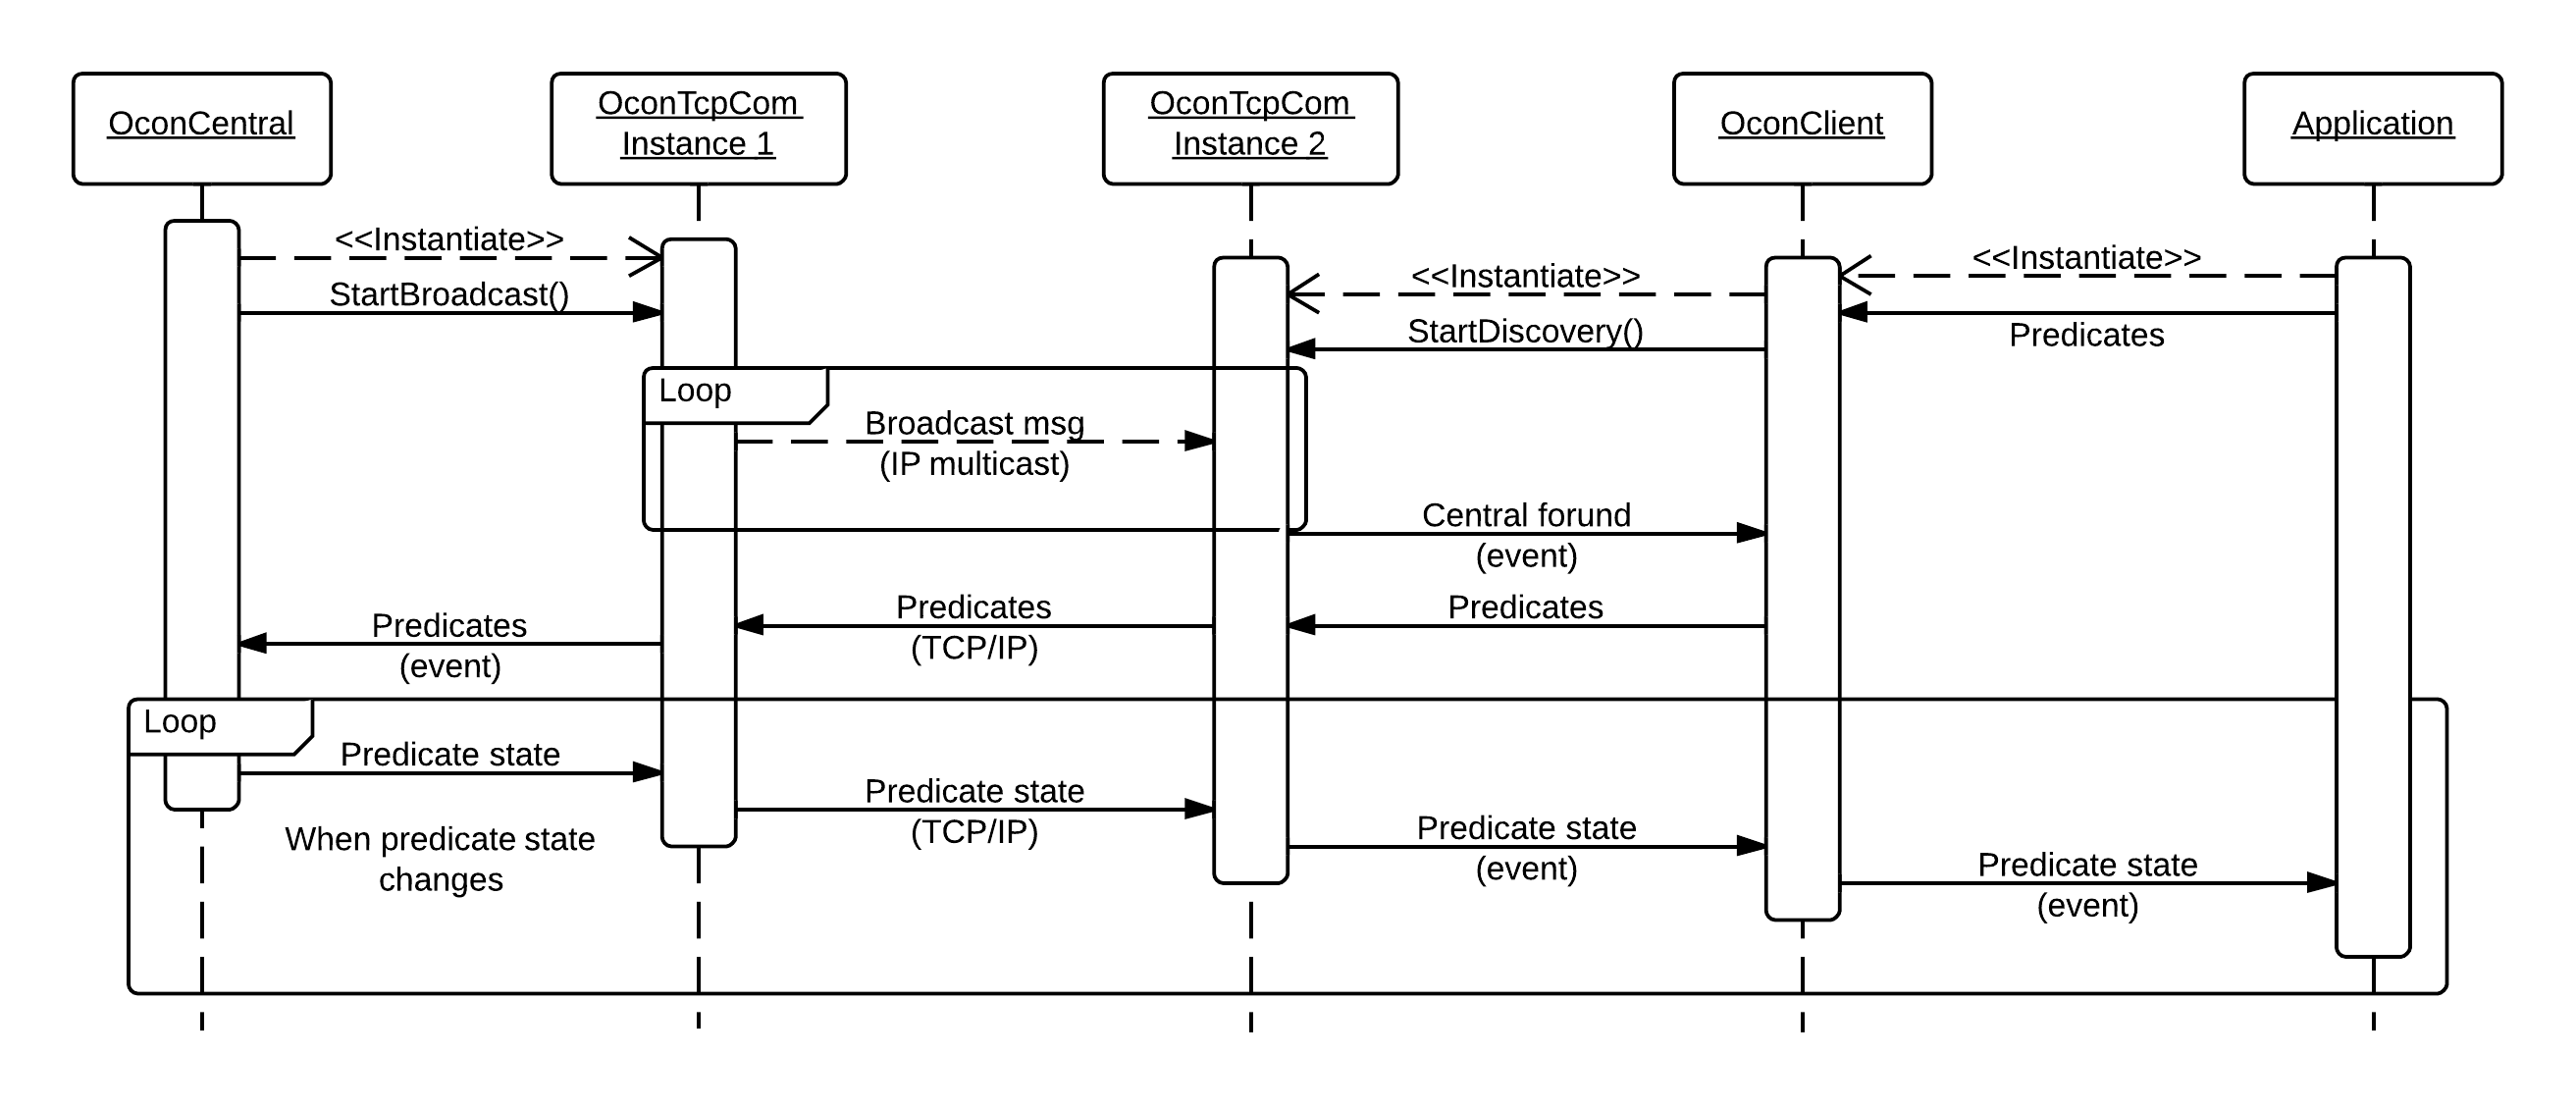
\includegraphics[width=\linewidth]{comHelperSequence-client.png}
\caption{Client to Central sequence diagram}
\label{fig:clientComHelper}
\end{figure}



\end{document}